\documentclass{article}
\title{CUDA Parallel Programming\\Homework 8}
\usepackage{graphicx}
\usepackage[UTF8]{ctex}
\usepackage{hyperref}
\usepackage{amsmath}
\usepackage{csvsimple}
\CTEXoptions[today=old]
\author{40647007S 朱健愷}

\begin{document}
	\maketitle
	\section{Source codes}
	\subsection{File Layout}
	\begin{itemize}
		\item Ising2D\textunderscore{NGPU}/ising2d\textunderscore{ngpu}\textunderscore{gmem}\textunderscore{v2}.cu - Main code computes the GPU accelerated Monte Carlo simulation of 2D ising model on a torus.
		\item Makefile - Script to auto generate executable from code.
		\item Ising2D\textunderscore{NGPU}/experiment.sh - Script to auto generate results of the GPU accelerated Monte Carlo simulation of 2D ising model on a torus. It test different block size setup on both 1GPU case and 2GPU case in simulation, and record their statistical result.
		\item Ising2D\textunderscore{NGPU}/experiment\textunderscore{1}.sh - Script to auto generate results of the GPU accelerated Monte Carlo simulation of 2D ising model on a torus. It test different temperature setup on both 1GPU case and 2GPU case in simulation using optimal block size get from experiment.sh, and record their statistical result.
		\item Ising2D\textunderscore{NGPU}/result/GPU\textunderscore* - Generated result using differeng GPU amount, the number behind "GPU" is the gpu amount I assigned to perform the experiment
		\item Ising2D\textunderscore{NGPU}/result/GPU\textunderscore*/block\textunderscore{*}/ - Generated result using differeng block size, the number behind "block" is the block size I assigned to perform the experiment.
		\item Ising2D\textunderscore{NGPU}/result/GPU\textunderscore*/T\textunderscore{*}/ - Generated result using differeng temperature, the number behind "T" is the temperature I assigned to perform the experiment.
		\item Ising2D\textunderscore{NGPU}/result/GPU\textunderscore*/block\textunderscore{*}/Output - Output the energy and magnetization density in every 100 sweeps.
		\item Ising2D\textunderscore{NGPU}/result/GPU\textunderscore*/block\textunderscore{*}/Output\textunderscore 2 - Output $\langle E\rangle$, $\delta E$, $\langle M\rangle$, $\delta M$ after applying autocorrelation function.
		\item Ising2D\textunderscore{NGPU}/result/GPU\textunderscore*/block\textunderscore{*}/ising2d\textunderscore{ngpu}\textunderscore{gmem}.dat - Output the energy and magnetization density in every 10 sweeps.
		\item Ising2D\textunderscore{NGPU}/result/GPU\textunderscore*/block\textunderscore{*}/spin\textunderscore{ngpu}\textunderscore{gmem}.dat - Output the final spin in each cell density.
		\item Ising2D\textunderscore{NGPU}/auto\textunderscore correlation/autoT\textunderscore B.c - The program to calculate the $\langle E\rangle$ and $\langle M\rangle$ and their $\delta E$, $\delta M$ after applying auto-correlation on them.

		\item notebook/*.png - Plots concluding output result
	\end{itemize}
	
	
	\subsection{Usage}
	Make code in both Ising2D\textunderscore{NGPU}/ directory
	Run the experiment.sh and experiment\textunderscore 1.sh script in Ising2D\textunderscore{NGPU}/ directory
	
	\begin{verbatim}
	cd Ising2D_NGPU
	make
	sh experiment.sh
	sh experiment_1.sh
	\end{verbatim}
	
	And it will produce the simulation result with different GPU amount, block size, and temperature.
	
	\section{Code design}
	In this assignment, I adopted the grid division technique learned in "solving laplacian equation in multi-GPU" to apply on this assignment. Firstly, I made the logic border of multi-GPU to be connected to its neighbor GPU using "enable peer access" in CUDA runtime library, and then use openMP to handle each GPU's execution and use "barrier" to synchronize their work, which prevent them from destroying the checkerboard scheme.
	
	There are two conditions that will break the checkerboard scheme, the first one is "Neighbor of current GPU and current GPU are running 'even' or 'odd' checkerboard scheme while the lattice dimension of them aren't even", this will cause the GPU to reference the changed spin of their neighbor. For this problem I simply prevent it assigning the lattice size that will cause this problem.
	
	The second one is "The synchornization problem", which means one GPU is running 'even' checkerboard scheme, while the other GPU already finished the 'even' checkerboard scheme and start running 'odd' checkerboard scheme, this will cause the GPU to reference the changed spin of their neighbor problem, too. For this problem I simply insert the openMP barrier to prevent them from running different scheme simultaneously.

	\section{Result}
	\subsection{Experiment environment}
	I ran my code on workstation provided in course, below is the Setup of workstation
	\begin{itemize}
		\item Operating system: Linux version 4.19.172 (root@twcp1)\\(gcc version 6.3.0 20170516 (Debian 6.3.0-18+deb9u1))
		\item CPU: Intel(R) Core(TM) i7-4790 CPU @ 3.60GHz
		\item GPU: Nvidia GTX 1060 6GB
		\item Memory: 32GB 
	\end{itemize}
	\subsection{Performance}
	Below two figures showed 1 GPU and 2 GPU processing time of monte carlo simulation of 2D ising model on the torus using different block size.
	\begin{figure}
		\centering
		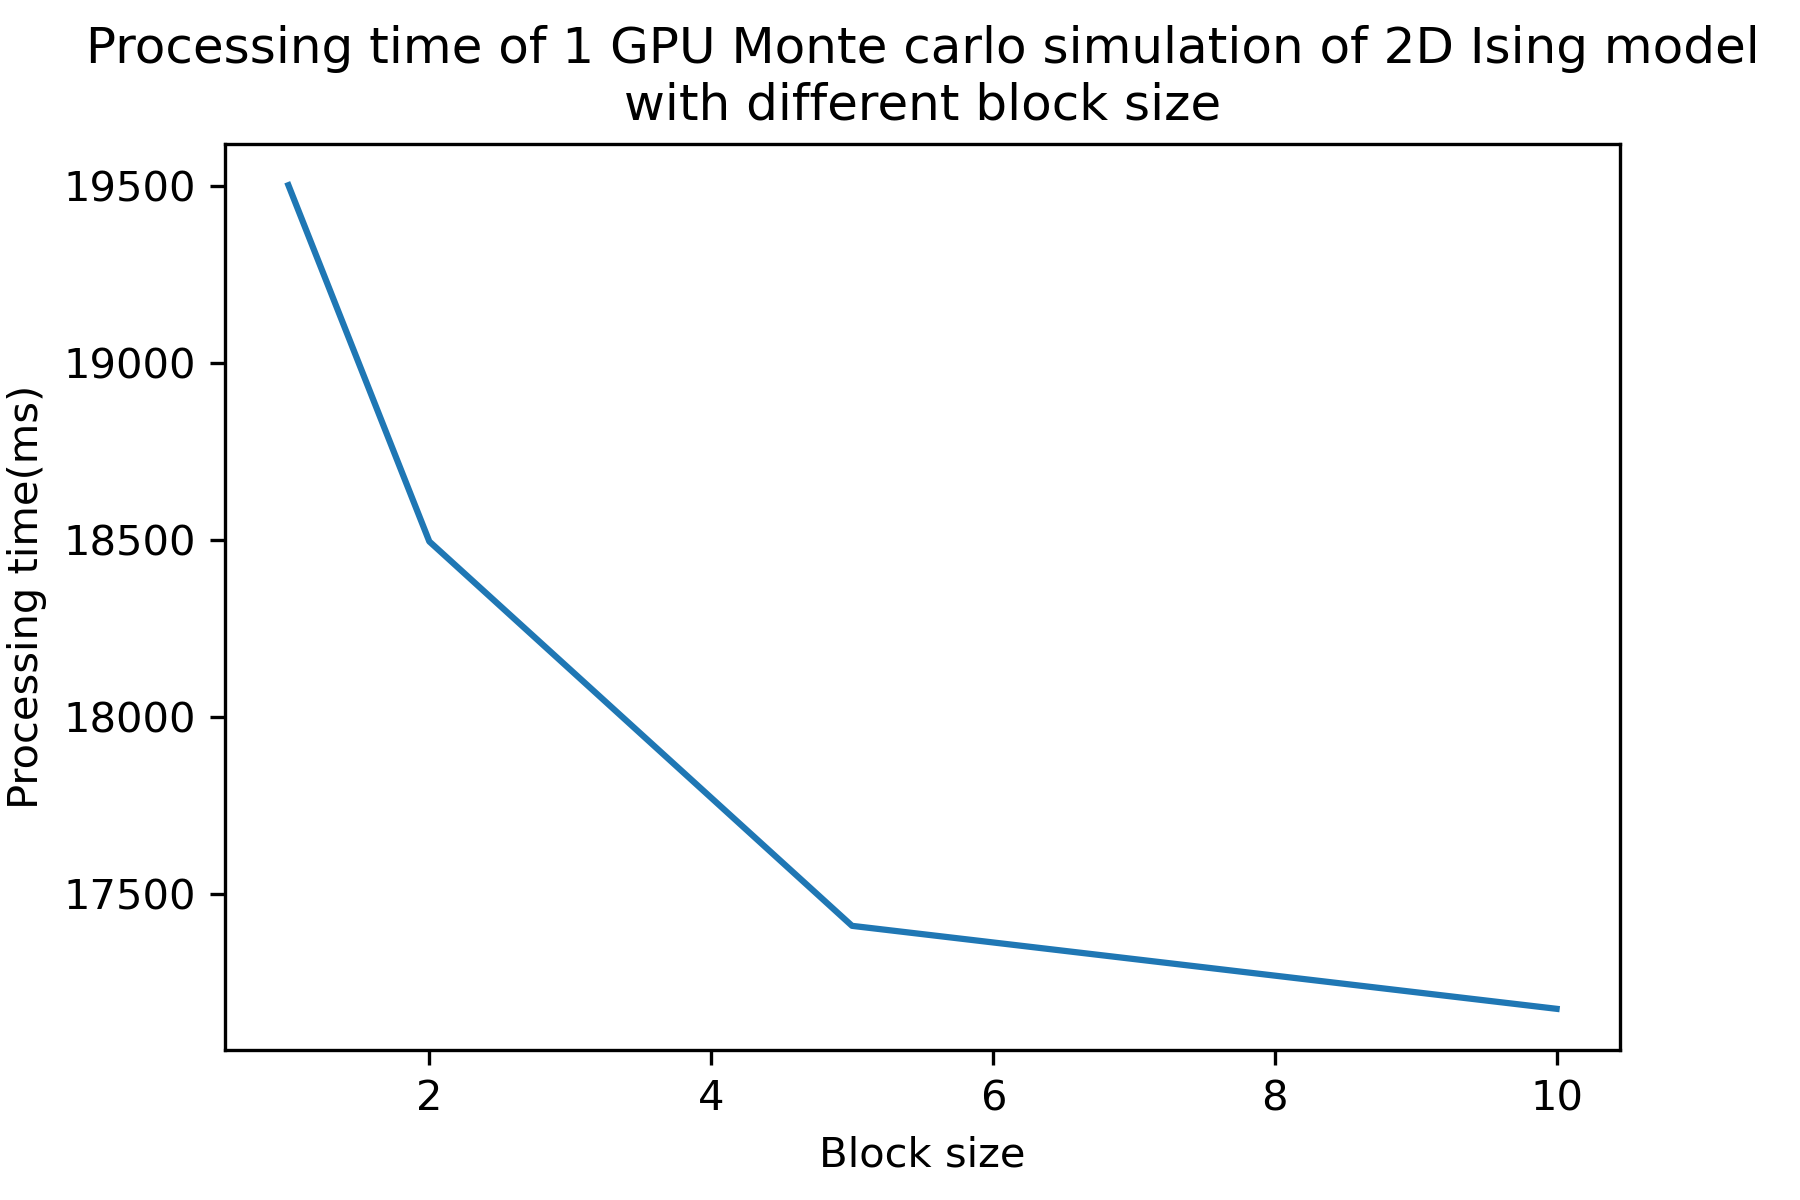
\includegraphics[width=0.9\linewidth]{notebook/1gpu_block}
	\end{figure}
	\begin{figure}
		\centering
		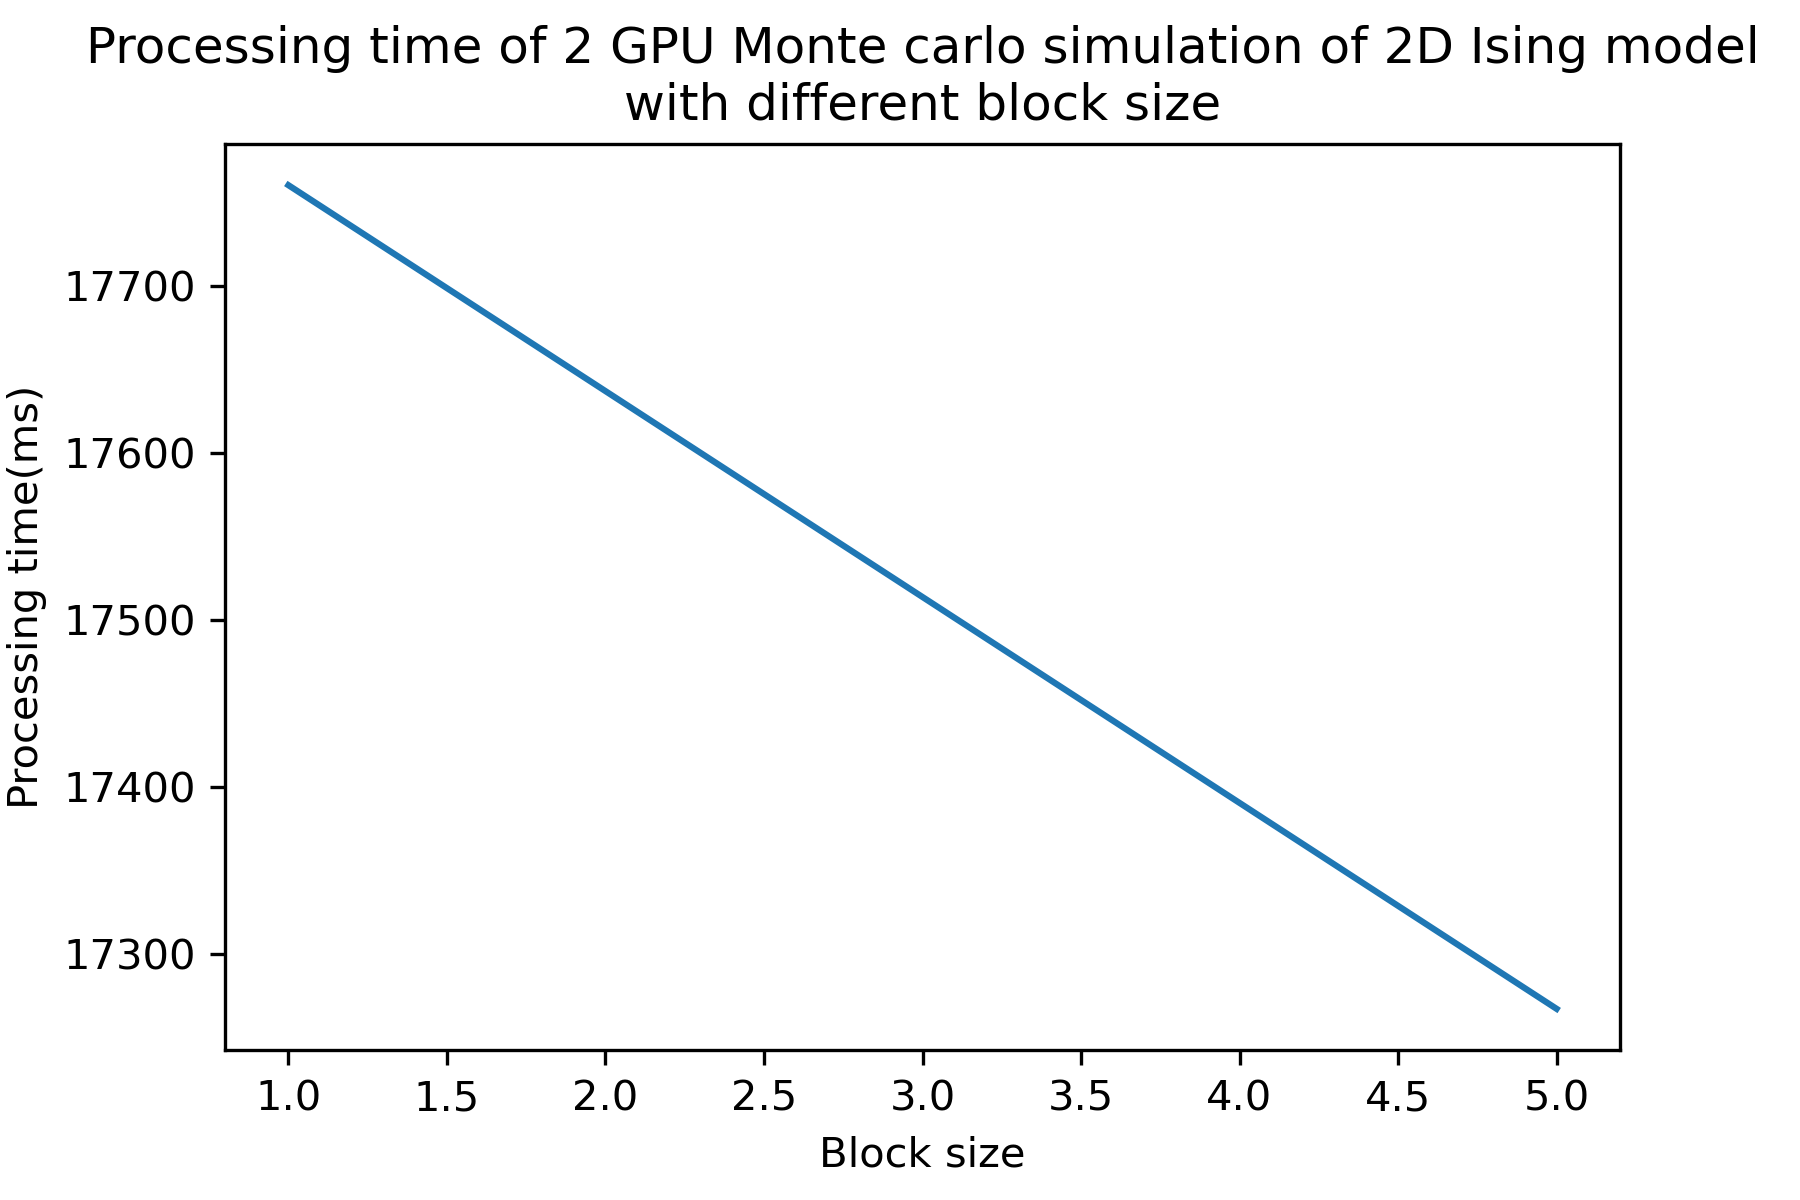
\includegraphics[width=0.9\linewidth]{notebook/2gpu_block}
	\end{figure}
	\newpage
	
	\subsection{Result plot}
	\subsubsection{1 GPU}
	Below two figures show the energy density and magnetization density using temperature=2.0

	Their $\langle E\rangle = -1.708829e+000 \pm 2.717343e-004$, $\langle M\rangle = -9.958487e-002 \pm 2.325785e-002$
	
	\begin{figure}[hb!]
		\centering
		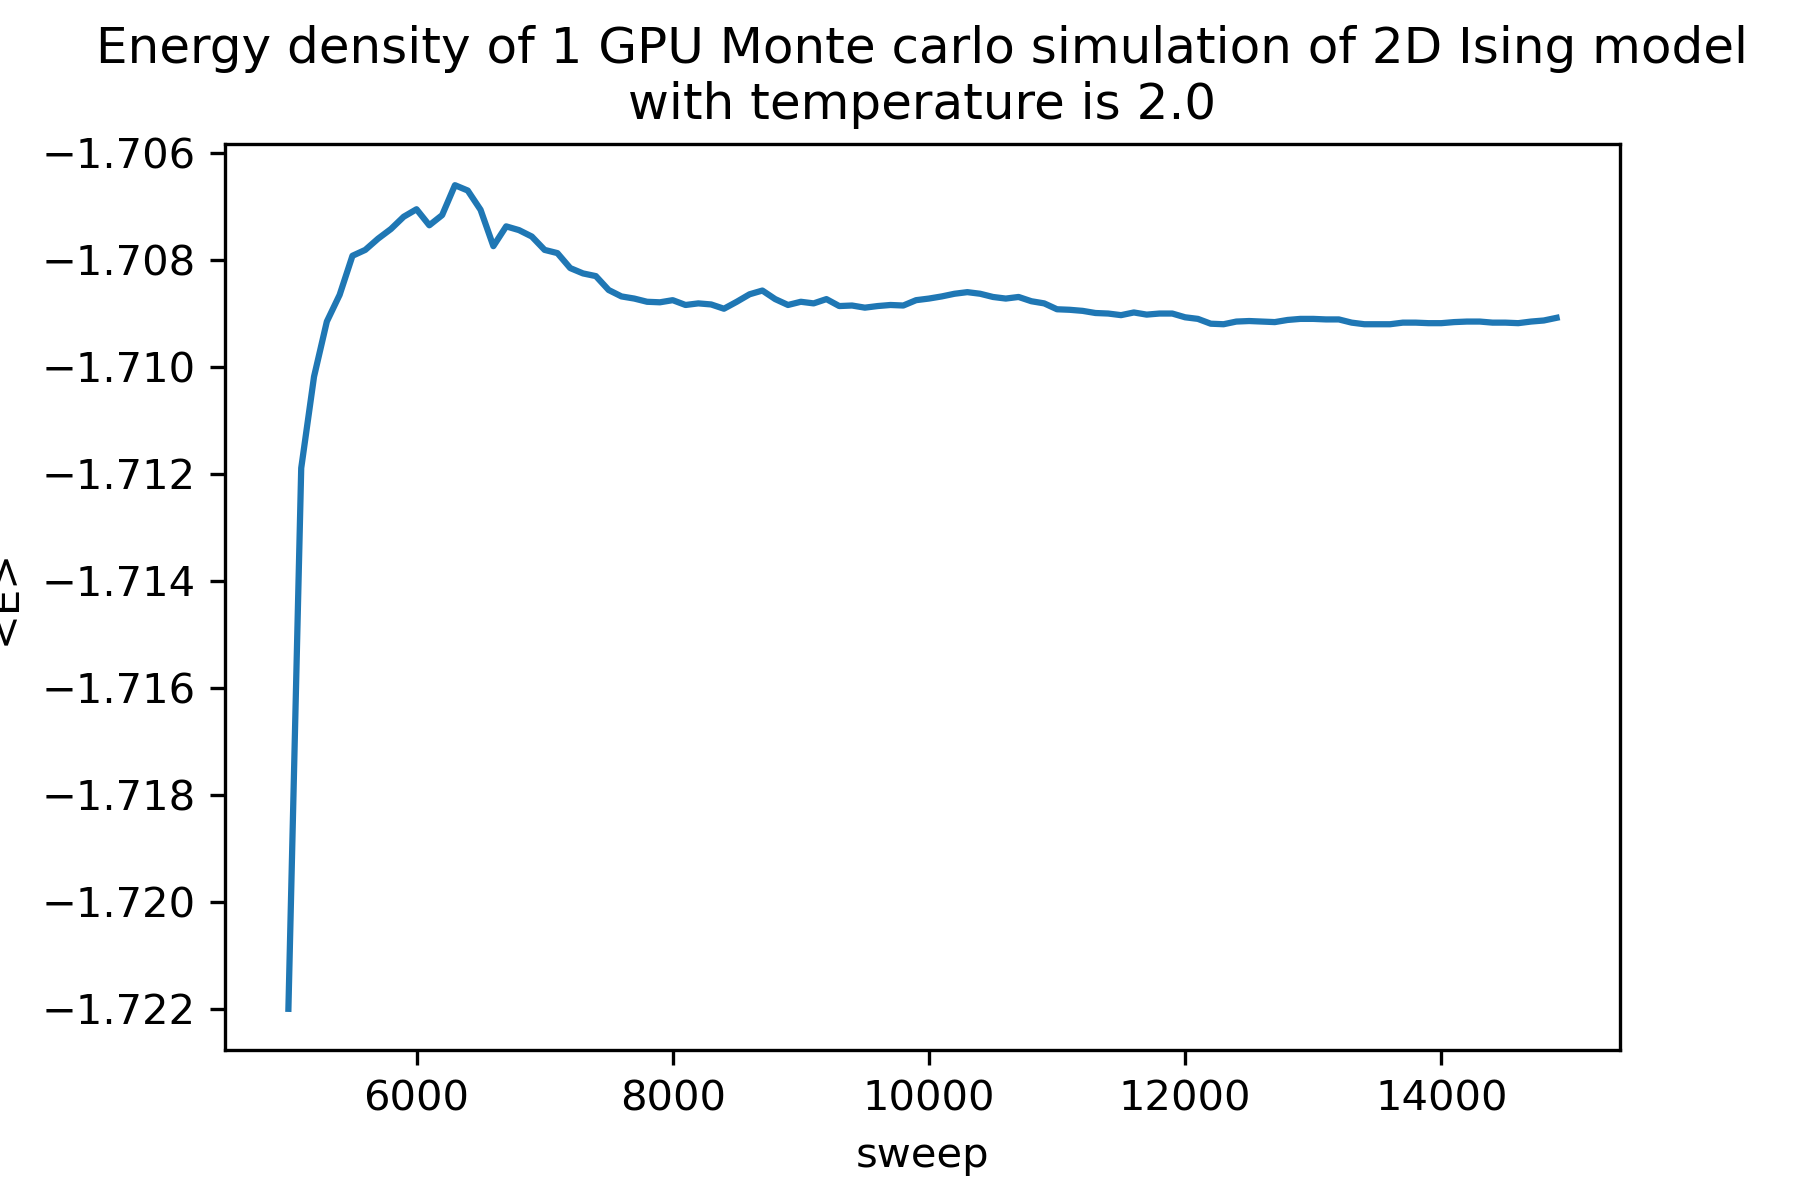
\includegraphics[width=0.8\linewidth]{notebook/1gpu_2.0_E}
	\end{figure}
	\begin{figure}[hb!]
		\centering
		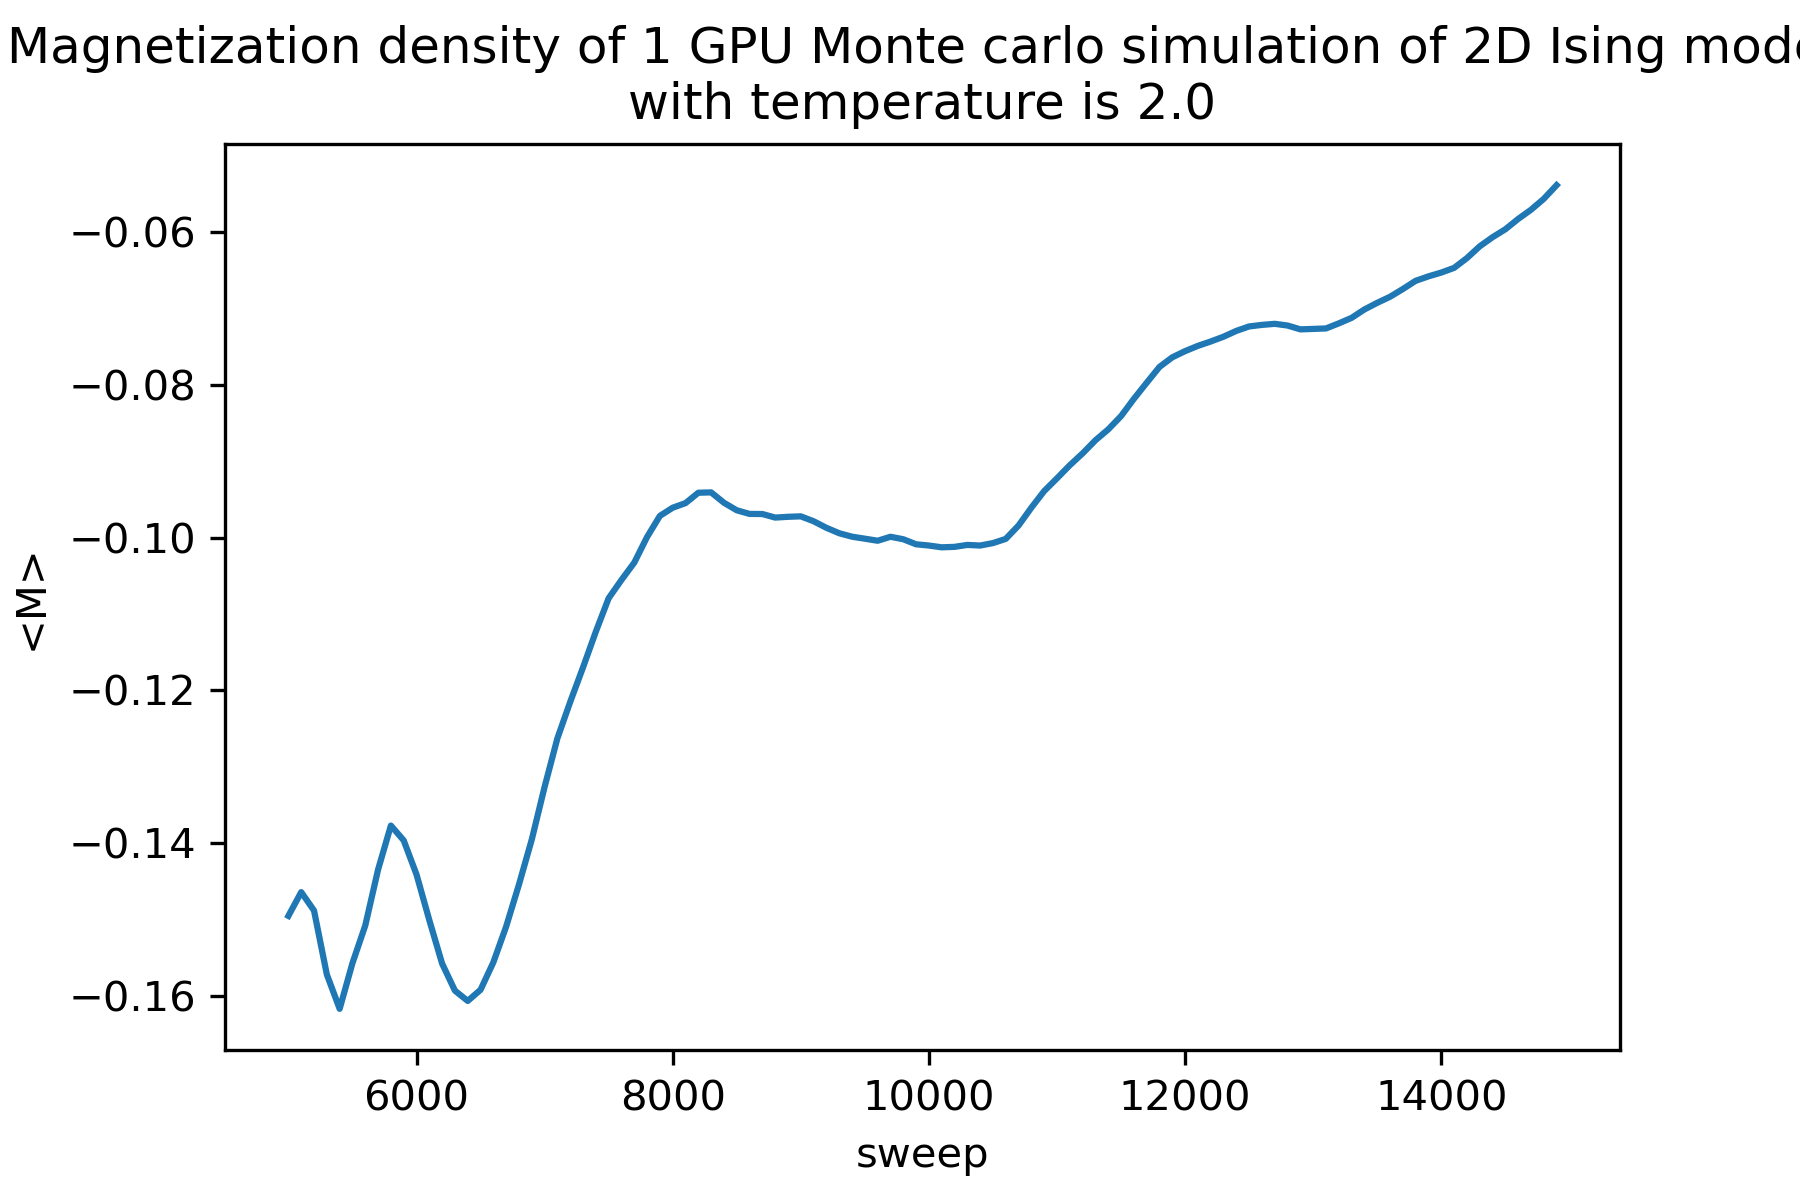
\includegraphics[width=0.8\linewidth]{notebook/1gpu_2.0_M}
	\end{figure}
	\newpage

	Below two figures show the energy density and magnetization density using temperature=2.3

	Their $\langle E\rangle = -1.344627e+000 \pm 1.485984e-003$, $\langle M\rangle = 1.220034e-001 \pm 3.549629e-002$

	\begin{figure}[hb!]
		\centering
		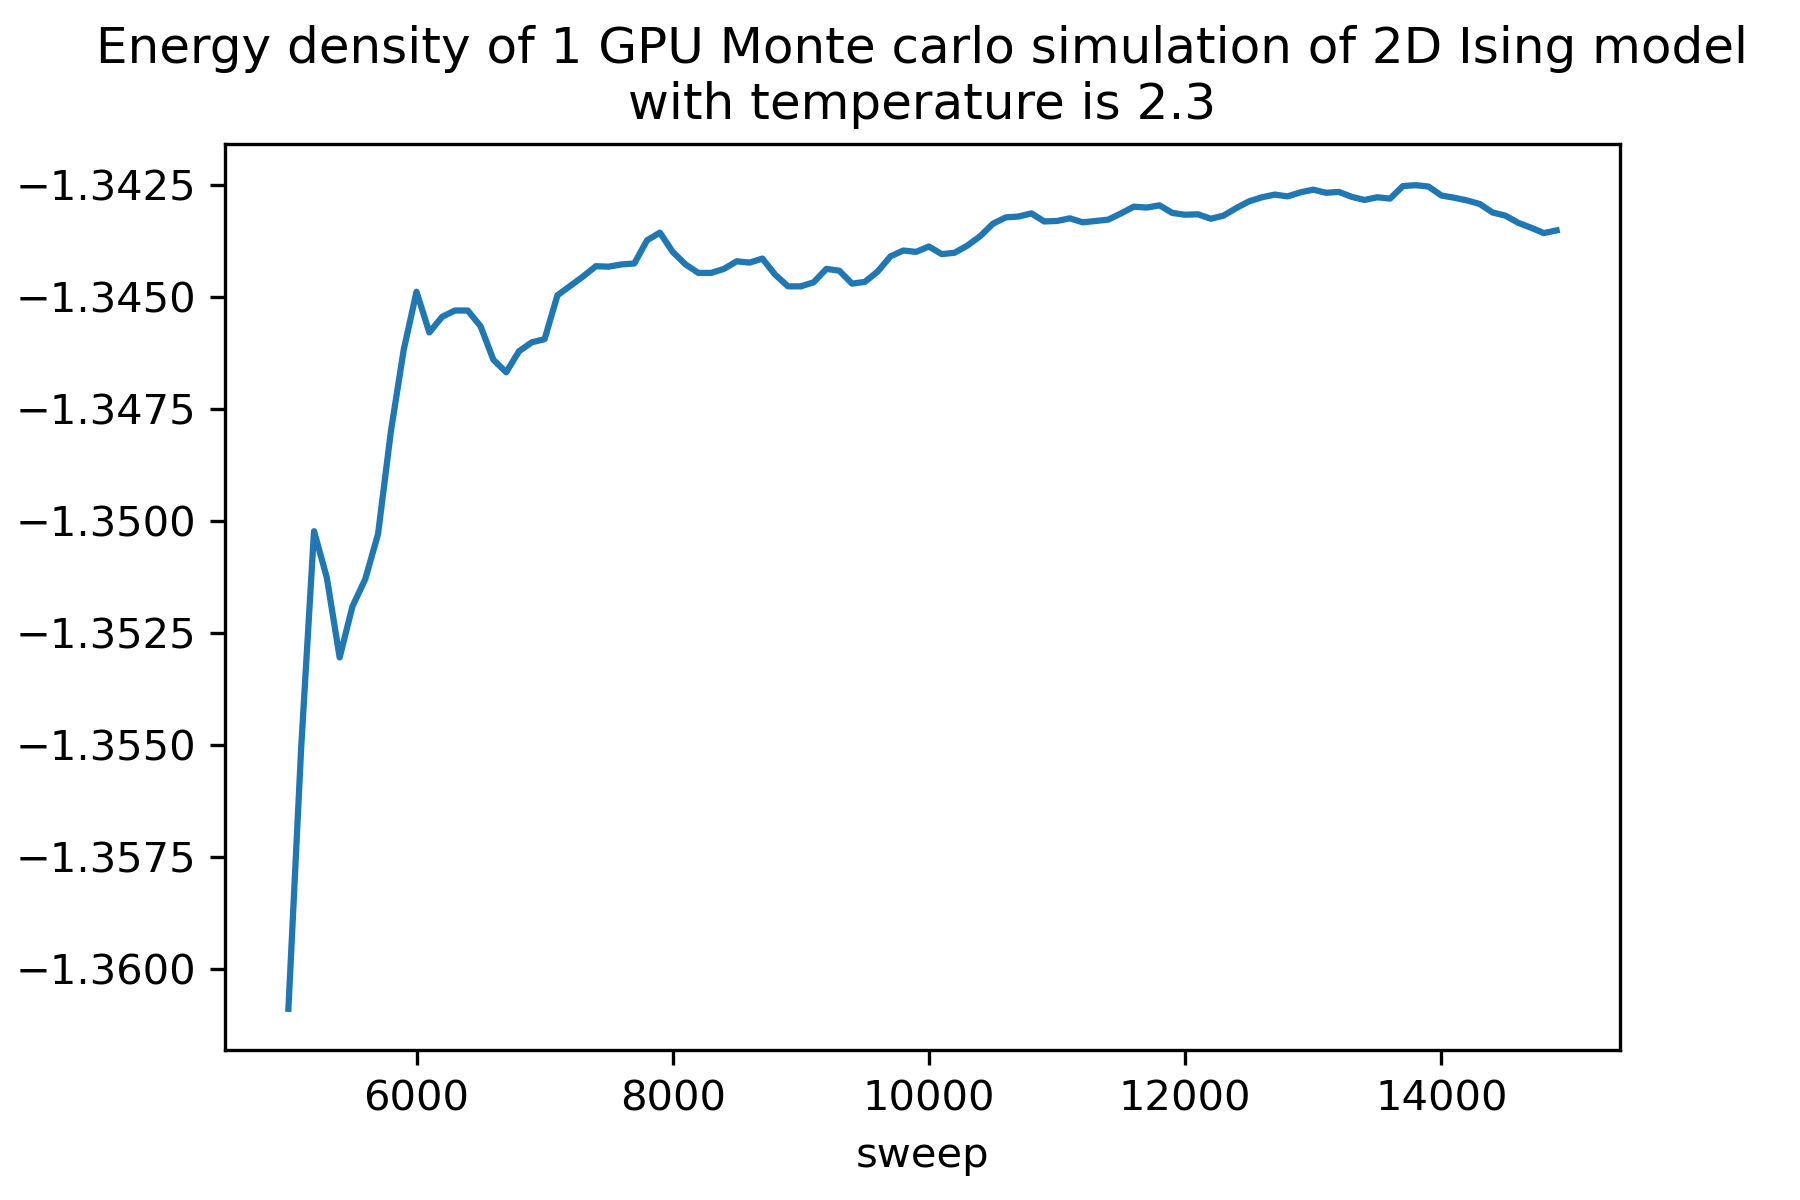
\includegraphics[width=0.9\linewidth]{notebook/1gpu_2.3_E}
	\end{figure}
	\begin{figure}[hb!]
		\centering
		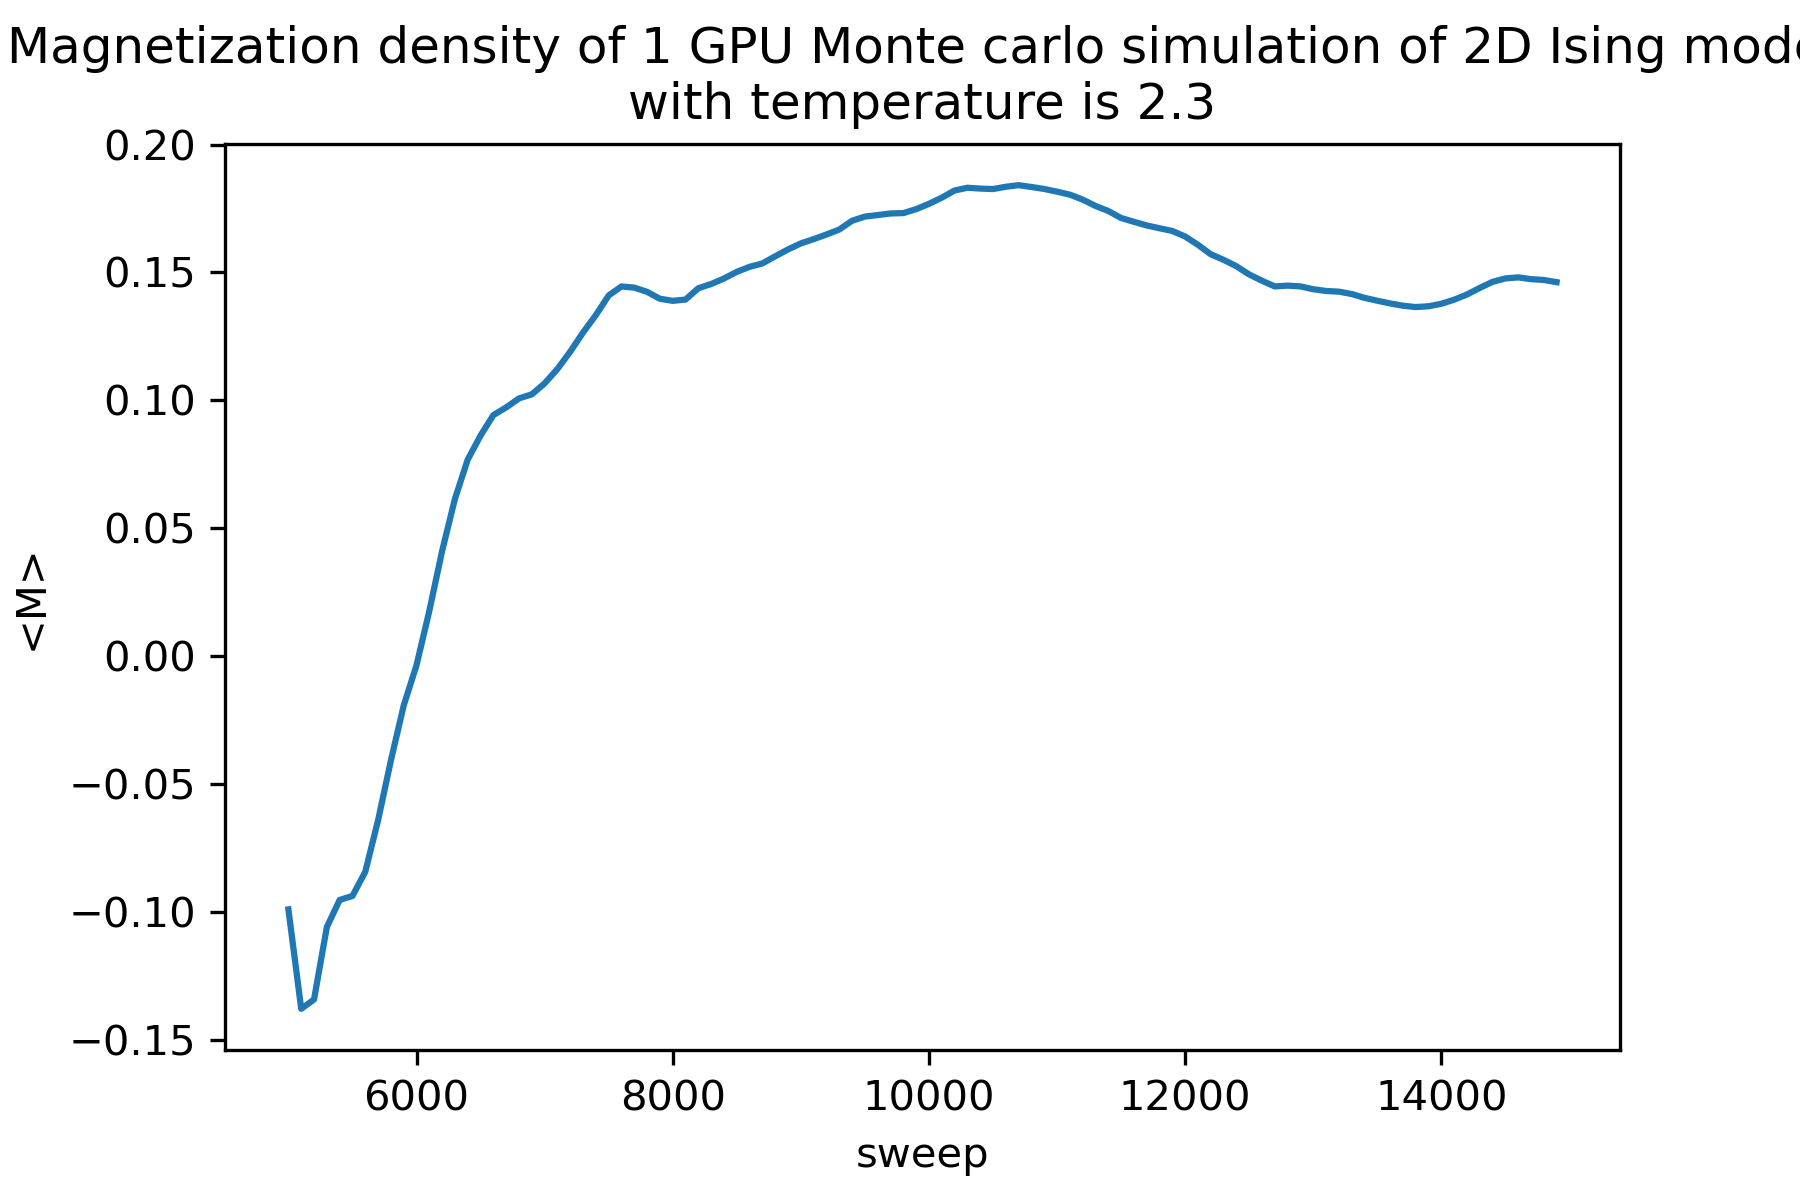
\includegraphics[width=0.9\linewidth]{notebook/1gpu_2.3_M}
	\end{figure}
	\newpage
	
	
	Below two figures show the energy density and magnetization density using temperature=2.4
	
	Their $\langle E\rangle = -1.203588e+000 \pm 2.851766e-004$, $\langle M\rangle = -1.539886e-002 \pm 3.005923e-003$
	
	\begin{figure}[hb!]
		\centering
		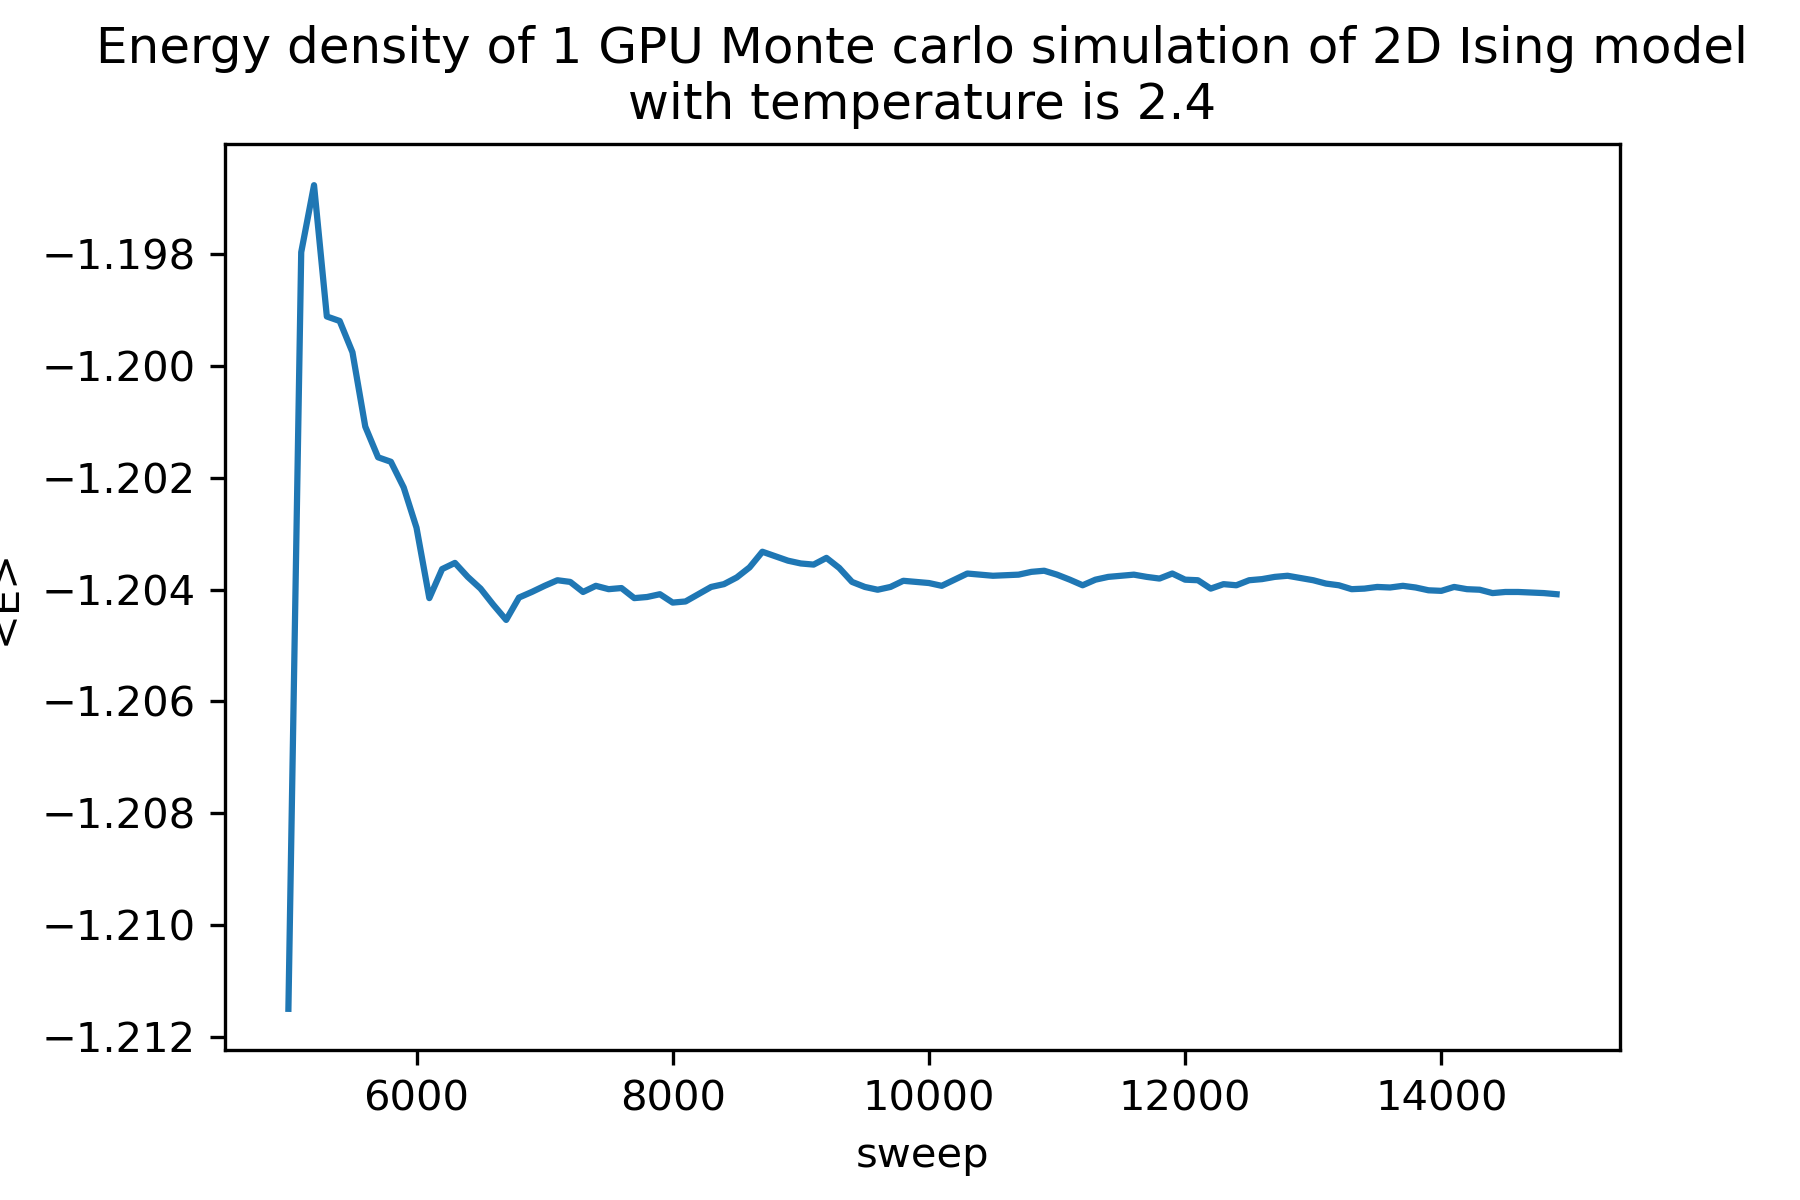
\includegraphics[width=0.9\linewidth]{notebook/1gpu_2.4_E}
	\end{figure}
	\begin{figure}[hb!]
		\centering
		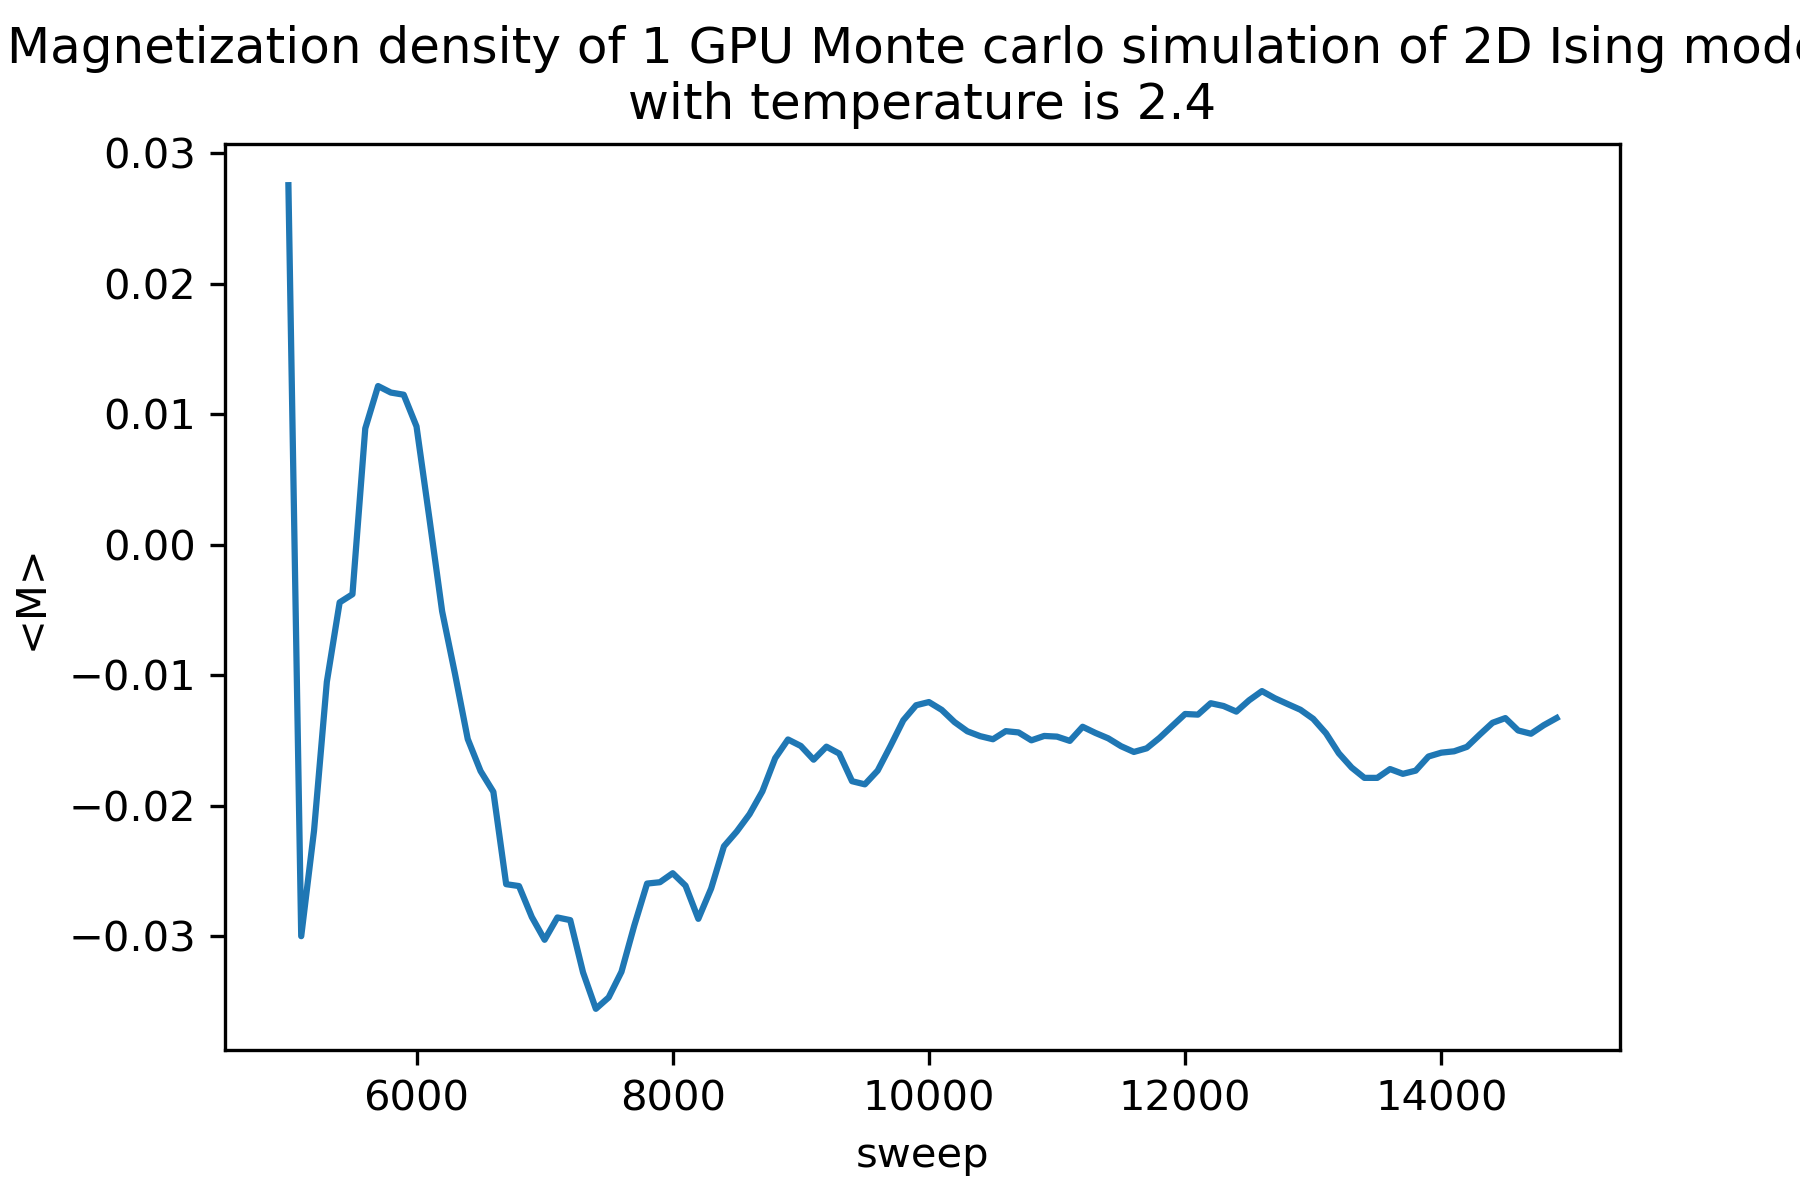
\includegraphics[width=0.9\linewidth]{notebook/1gpu_2.4_M}
	\end{figure}
	\newpage

	The other simulation figures using different temperature can be found in notebook/ directory, which format is 1gpu\textunderscore{\textlangle temperature\textrangle}\textunderscore[E][M],
	where "E" and "M" indicate the figure showing the energy density of magnetization density.

	\subsubsection{2 GPU}
	Below two figures show the energy density and magnetization density using temperature=2.1

	Their $\langle E\rangle = -1.661916e+000 \pm 3.137847e-004$, $\langle M\rangle = -8.686338e-001 \pm 1.927622e-004$

	\begin{figure}[hb!]
		\centering
		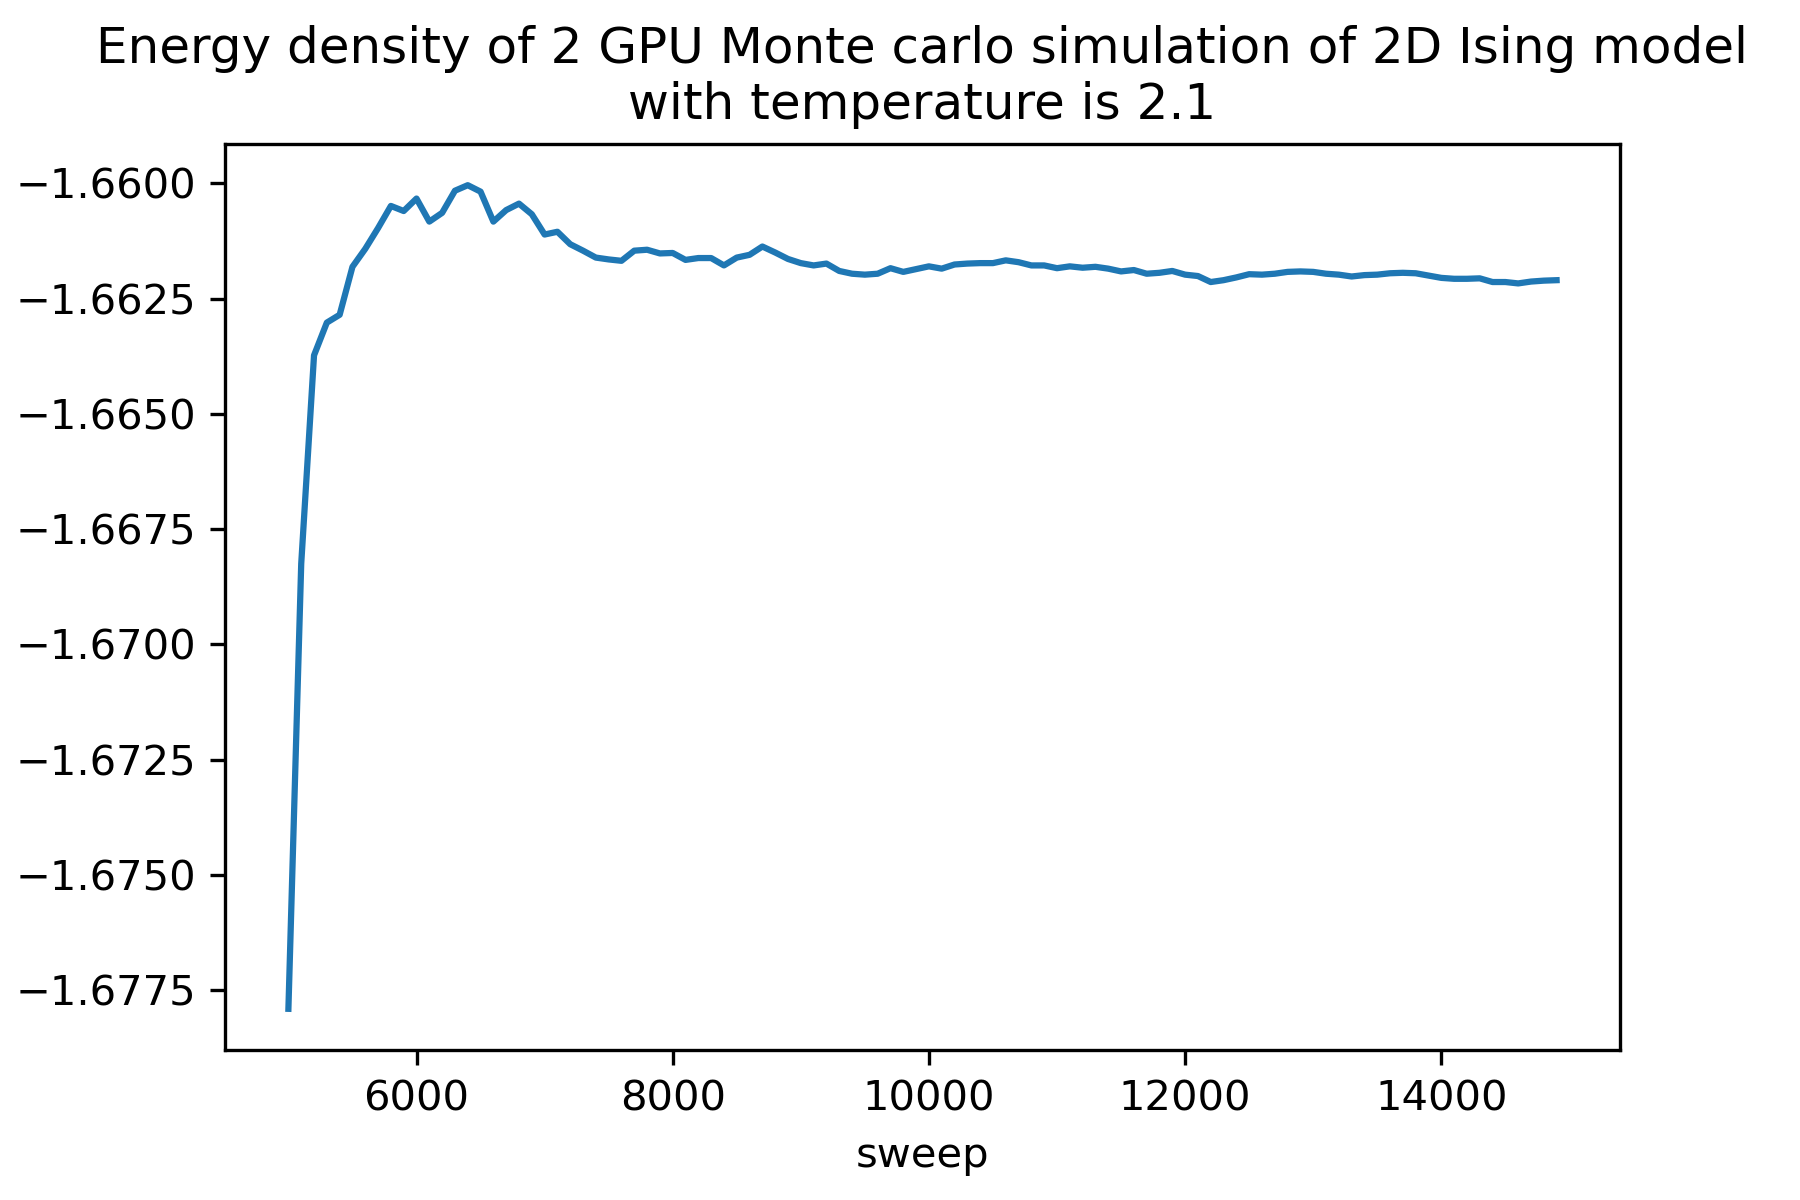
\includegraphics[width=0.7\linewidth]{notebook/2gpu_2.1_E}
	\end{figure}
	\begin{figure}[hb!]
		\centering
		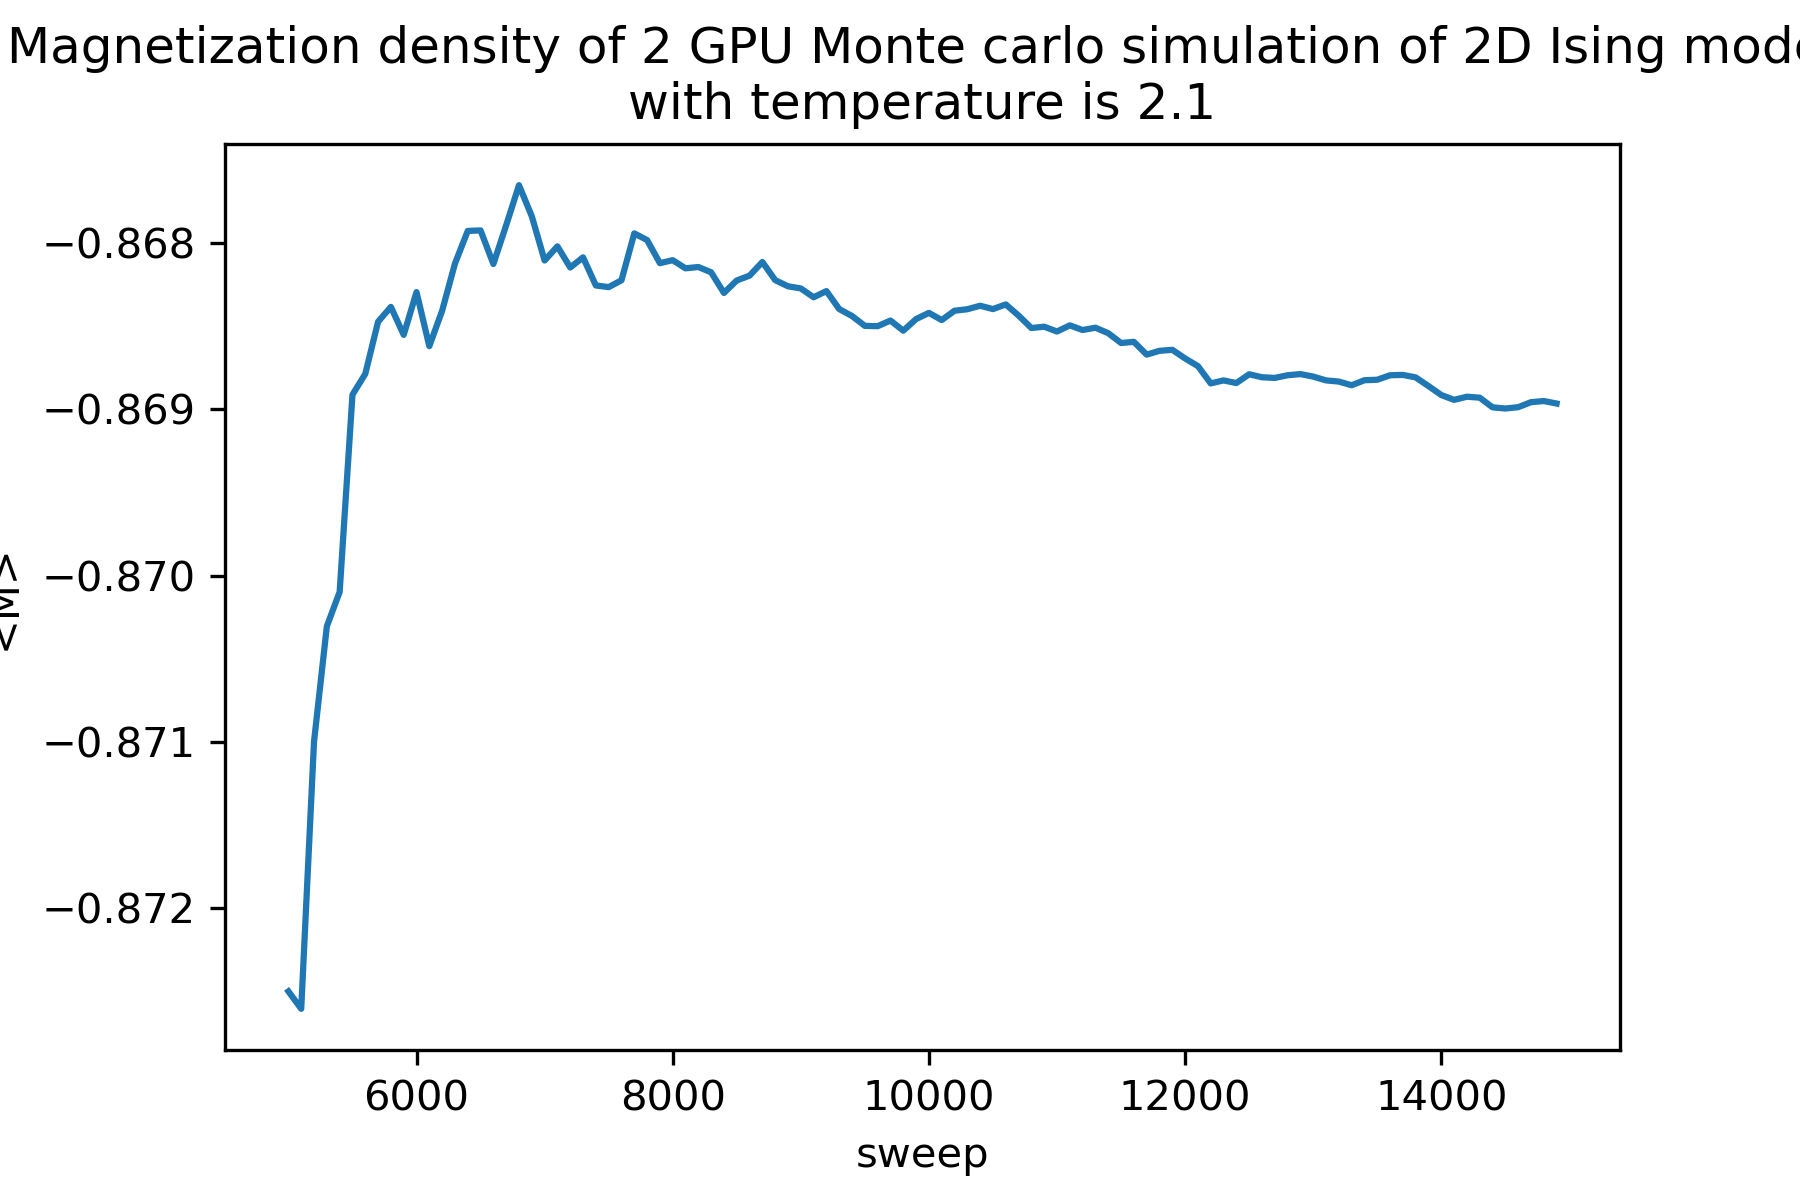
\includegraphics[width=0.7\linewidth]{notebook/2gpu_2.1_M}
	\end{figure}
	\newpage
	
	Below two figures show the energy density and magnetization density using temperature=2.2

	Their $\langle E\rangle = -1.545266e+000 \pm 7.267663e-004$, $\langle M\rangle = -7.833565e-001 \pm 1.346352e-003$

	\begin{figure}[hb!]
		\centering
		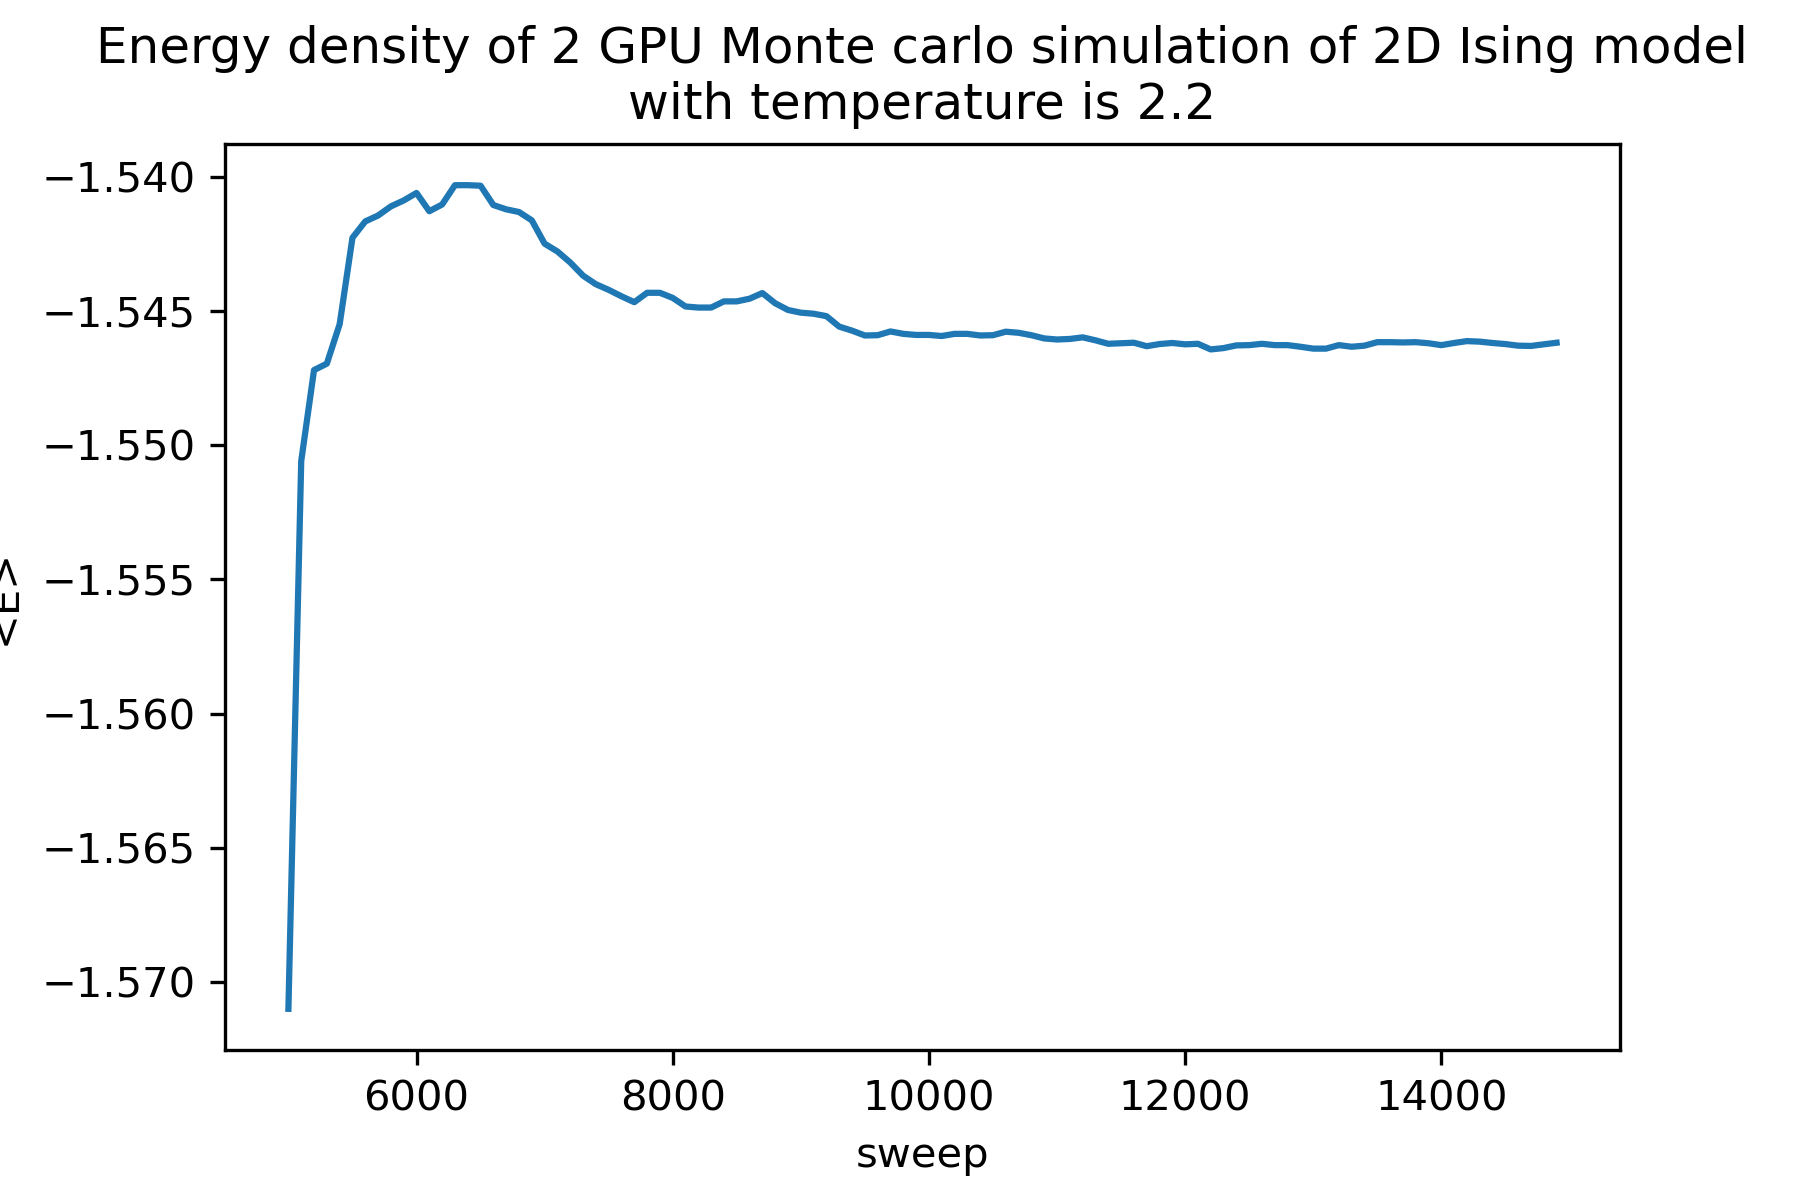
\includegraphics[width=0.9\linewidth]{notebook/2gpu_2.2_E}
	\end{figure}
	\begin{figure}[hb!]
		\centering
		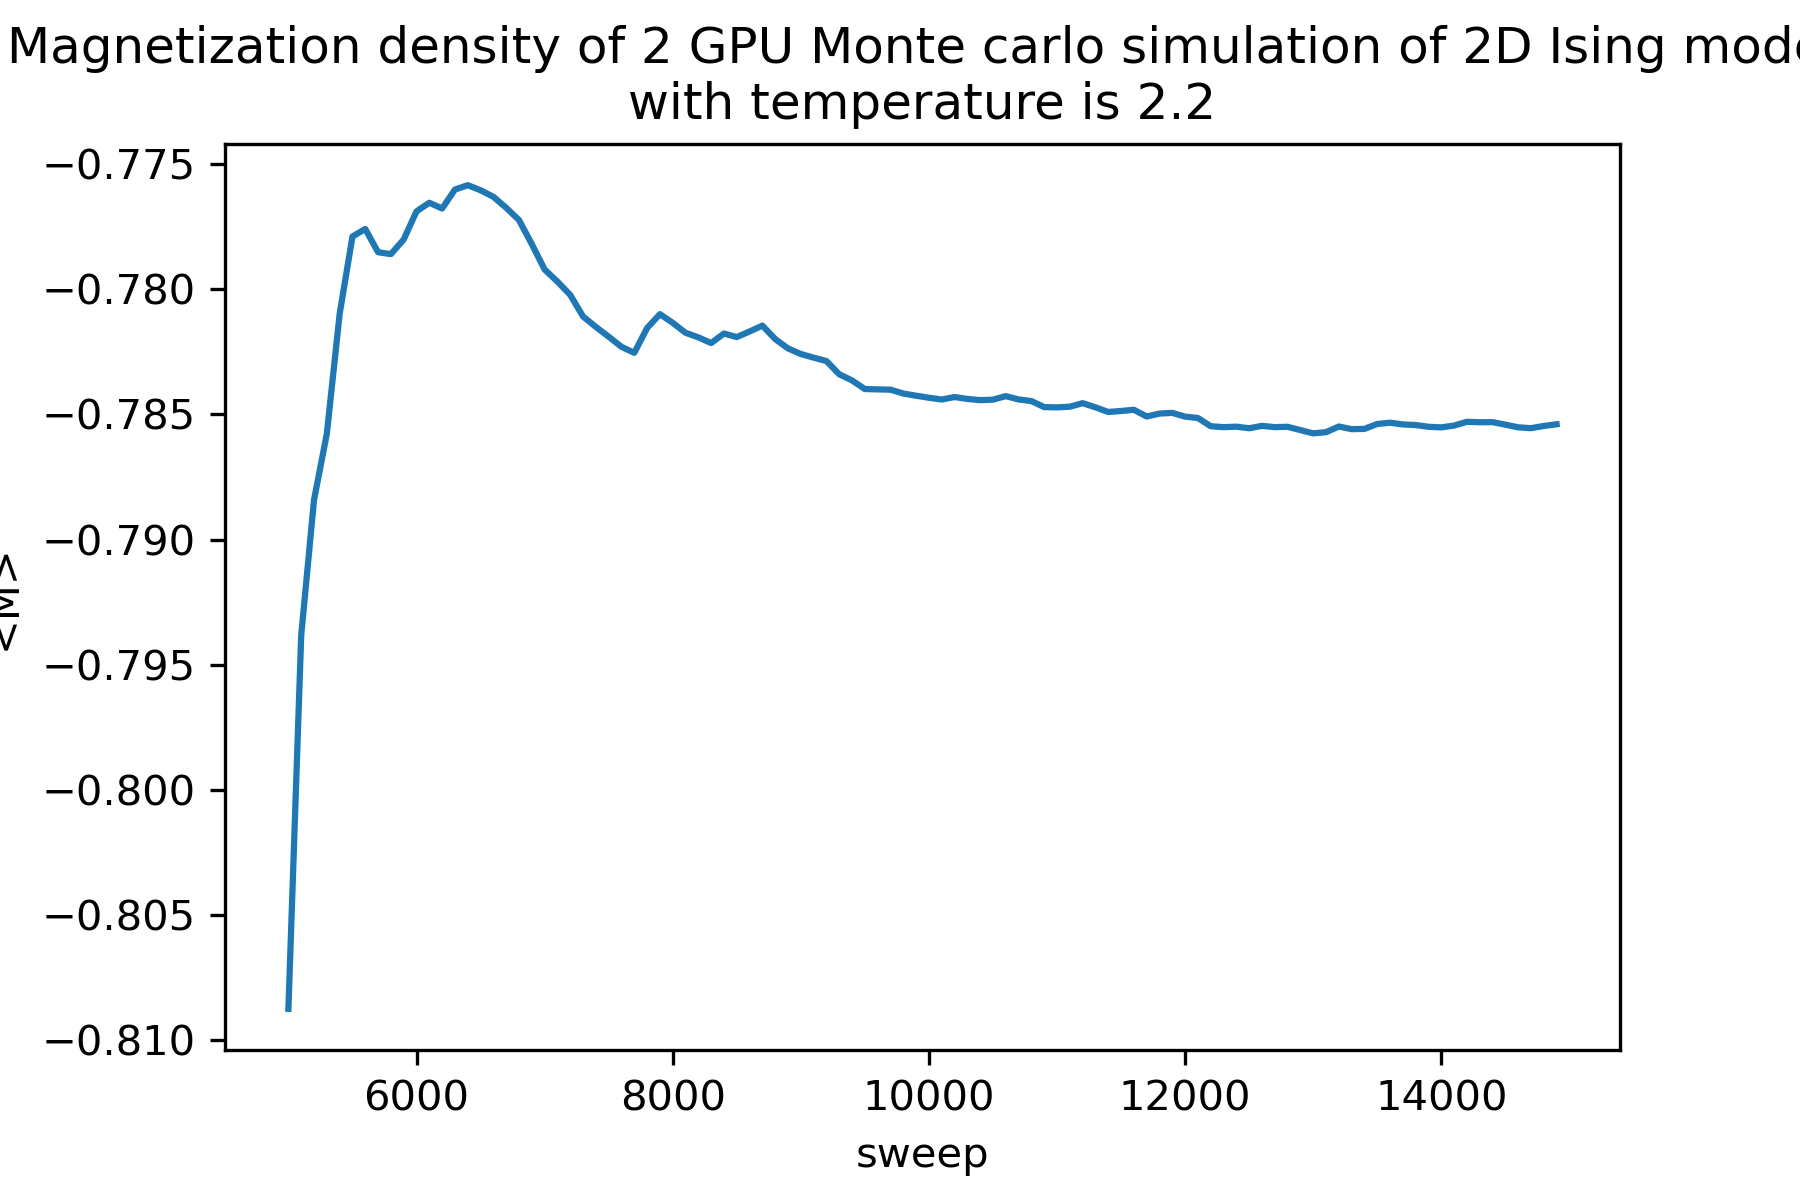
\includegraphics[width=0.9\linewidth]{notebook/2gpu_2.2_M}
	\end{figure}
	
	Below two figures show the energy density and magnetization density using temperature=2.5

	Their $\langle E\rangle = -1.105536e+000 \pm 7.271165e-004$, $\langle M\rangle = 3.581217e-003 \pm 1.653809e-003$

	\begin{figure}[hb!]
		\centering
		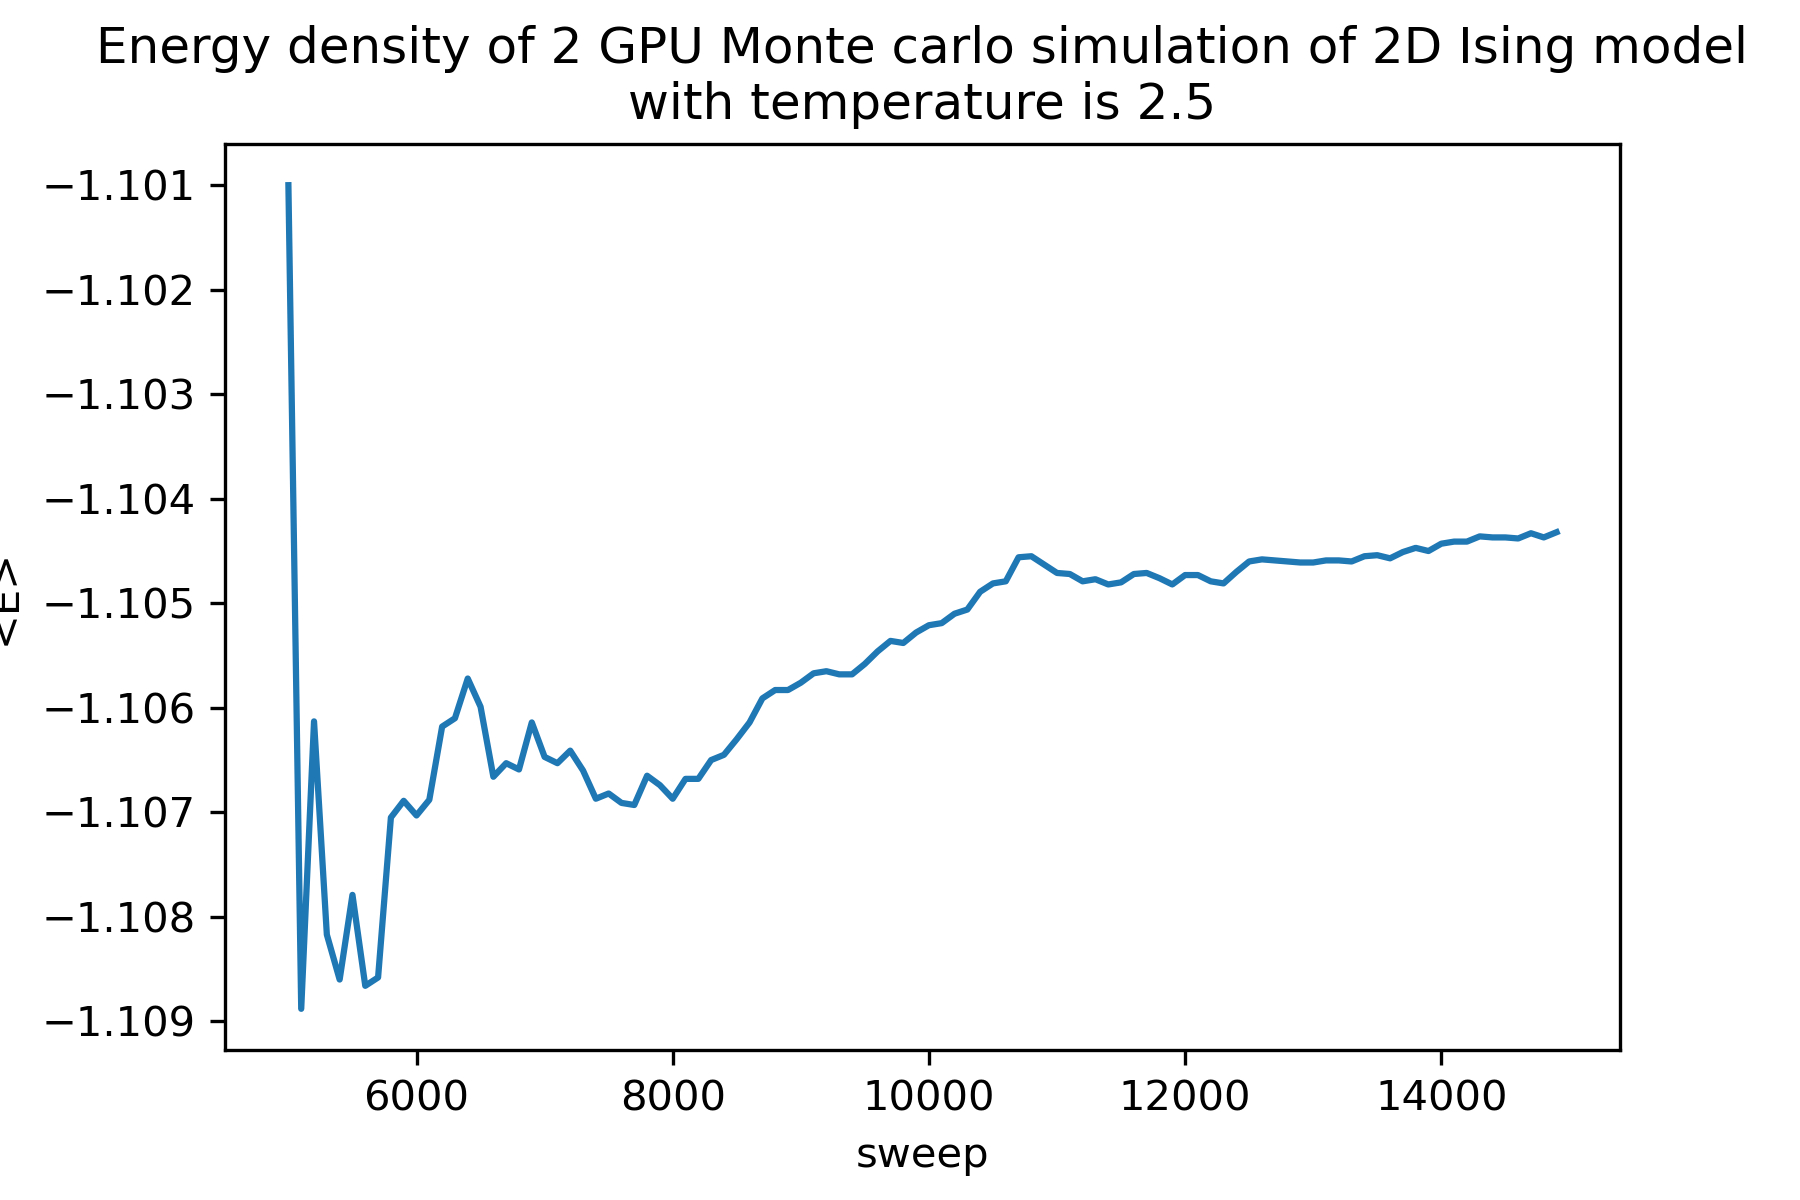
\includegraphics[width=0.9\linewidth]{notebook/2gpu_2.5_E}
	\end{figure}
	\begin{figure}[hb!]
		\centering
		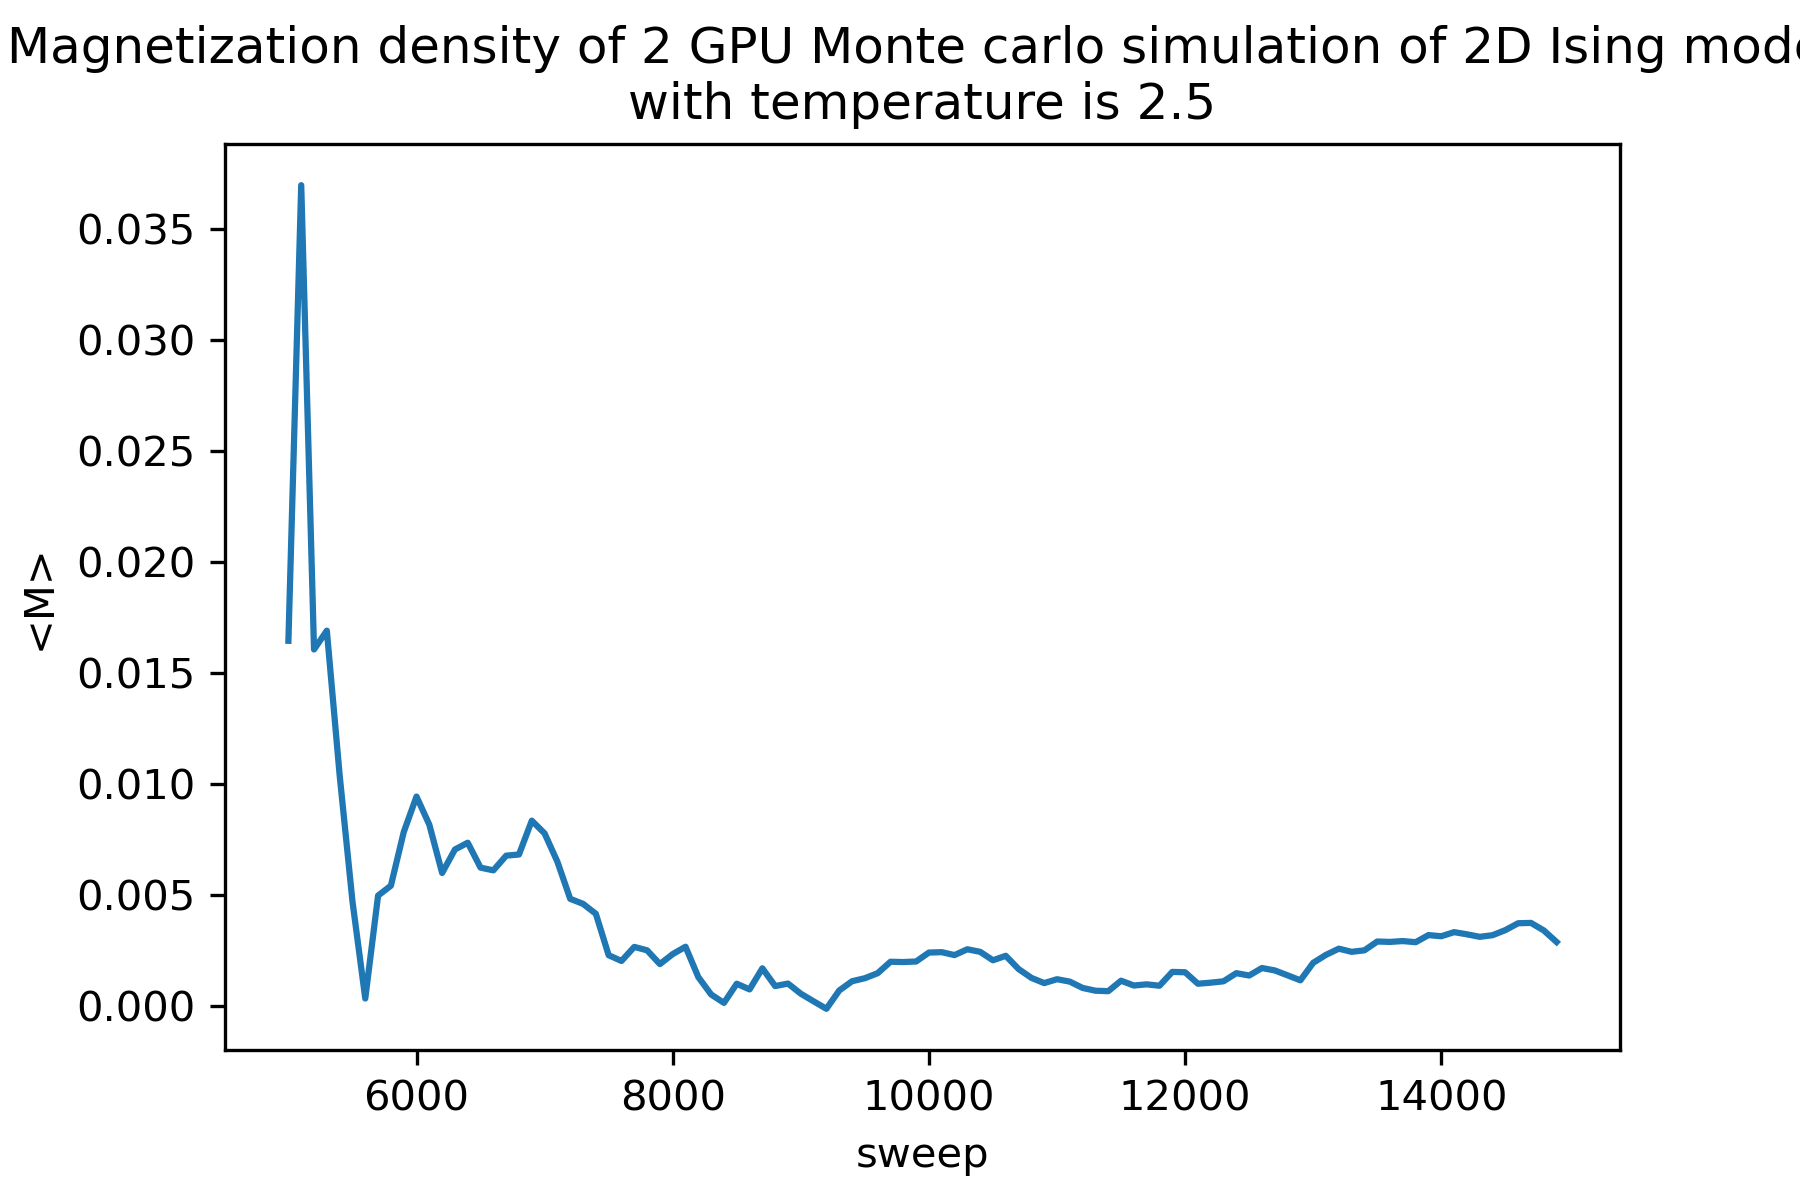
\includegraphics[width=0.9\linewidth]{notebook/2gpu_2.5_M}
	\end{figure}	

	The other simulation figures using different temperature can be found in notebook/ directory, which format is 2gpu\textunderscore{\textlangle temperature\textrangle}\textunderscore[E][M],
where "E" and "M" indicate the figure showing the energy density of magnetization density.
	
	\newpage
	Below figure shows absolute magnetization over different temperature.
	
	\begin{figure}[hb!]
		\centering
		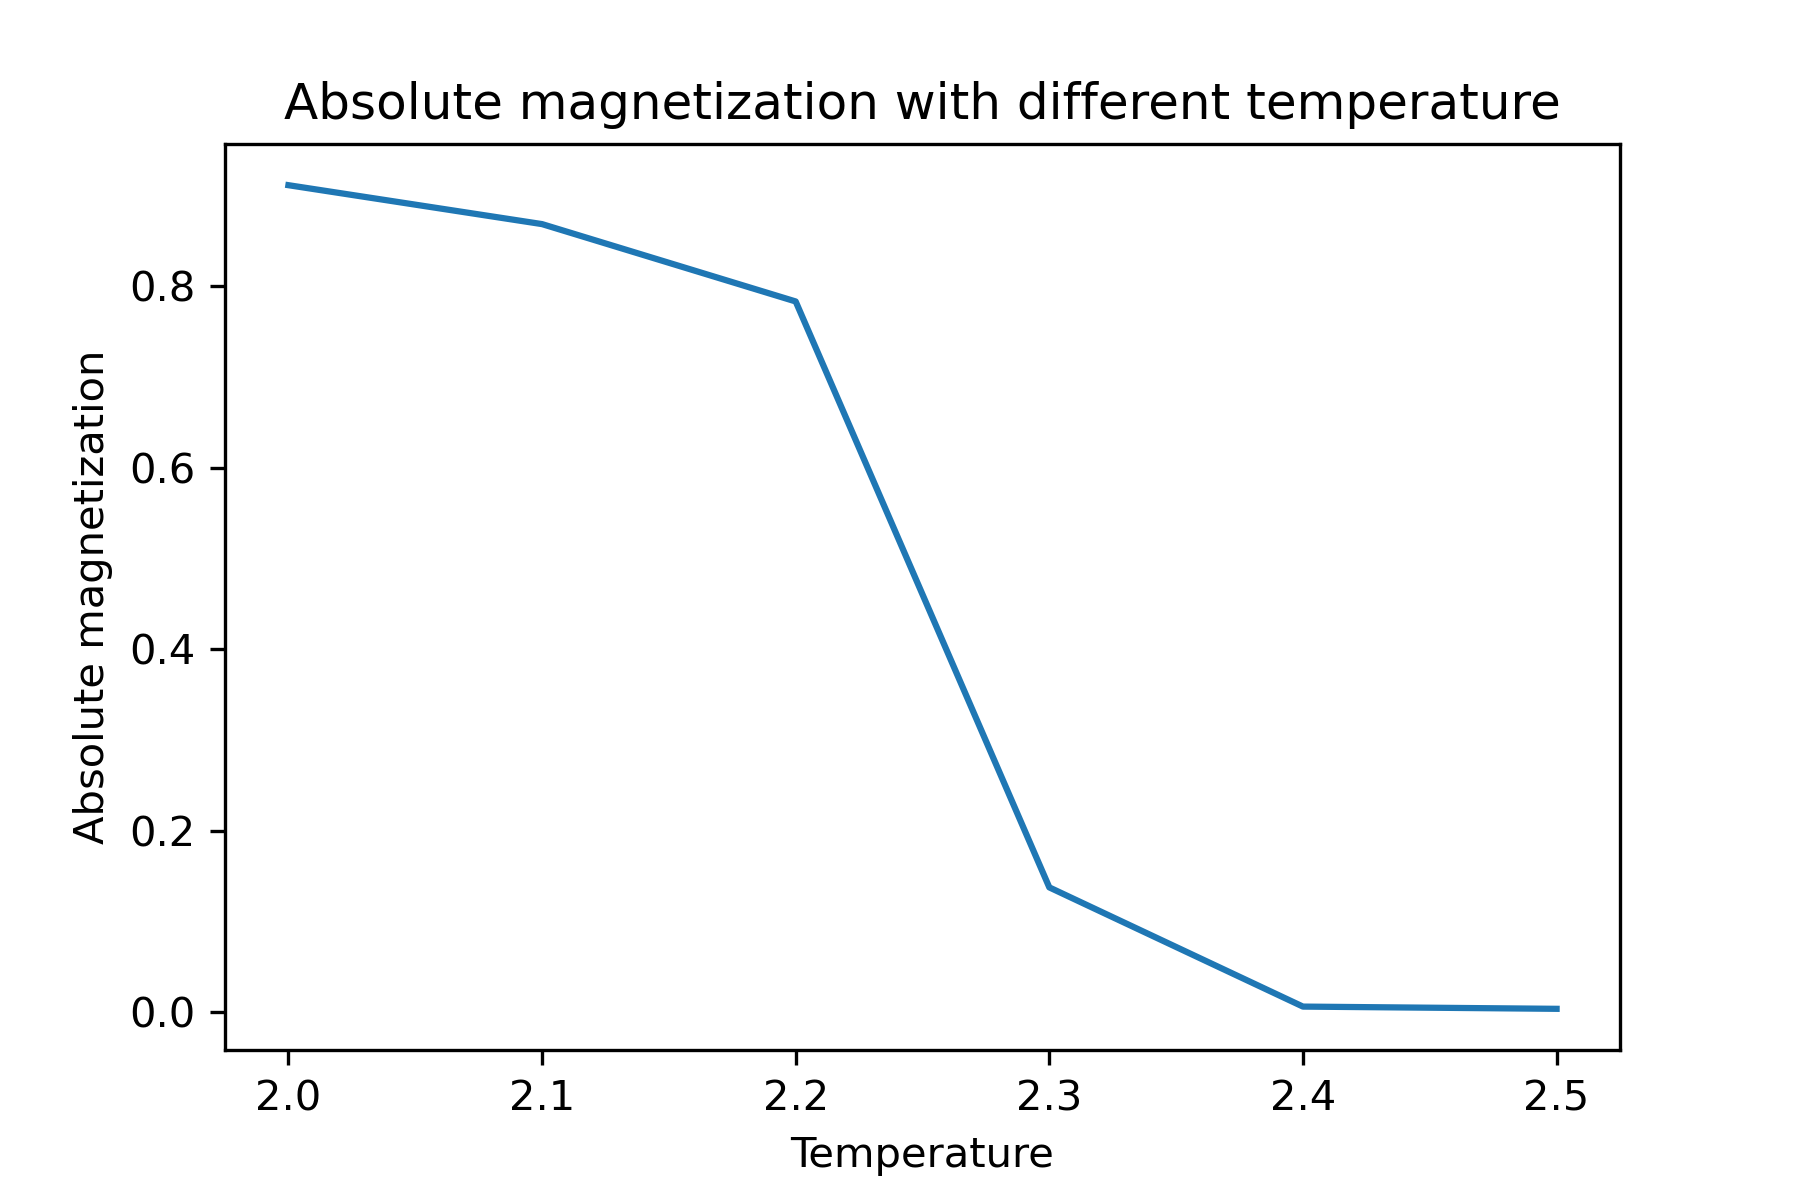
\includegraphics[width=0.9\linewidth]{notebook/2gpu_absolute_magnetization}
	\end{figure}	
	
	\subsection{Observation}
	The 2 GPU case is faster than 1 GPU case of monte carlo simulation of 2D ising model on the torus in all of the plausible block size 2 GPU case can use, but due to the checkerboard scheme's limitation, I can't test more block size to get more accurate data on other block size setup for 2 GPU case.
	
	From the figure shown above, we can see that after long time(sweeps) both the energy density and magnetization density gets stable eventually. 
	
	The absolute magnetization over different temperature figure approximately agree with Onsager's solution with no applied external magnetic field.
	
	\section{Reference}
	\href{https://www.hiskp.uni-bonn.de/uploads/media/ising_II.pdf}{Numerical Analysis of 2-D
		Ising Model}
	
	\href{https://phas.ubc.ca/~berciu/TEACHING/PHYS503/PROJECTS/05_dominic.pdf}{Classical Monte Carlo and the Metropolis Algorithm:
	Revisiting the 2D Ising Model}
\end{document}